\chapter{Measurement Results}
\label{ch:results}

In this chapter we present and discuss the measurement results for different combinations of MAC protocols employed on the two links.  We first assess the measurement results where both senders employ the same MAC protocols. Subsequently, we do the same for several combinations of different MAC protocols. 

\section{Same MAC Protocol For Both Links}
\label{sec:same-protocols}

For the results presented tfhroughout this section, both transmitters executed identical flowgraphs. Generally, when both links use the same MAC protocol we expect to see comparable results for each link over a sufficiently longer period of time, although small variations are also expected due to statistical and hardware-related effects and inaccuracies. 

\subsection{ALOHA}
\label{sec:dbl-aloha}

\begin{figure}[tb]
	\label{fig:results-aloha-dbl-throughput}
	\begin{center}
		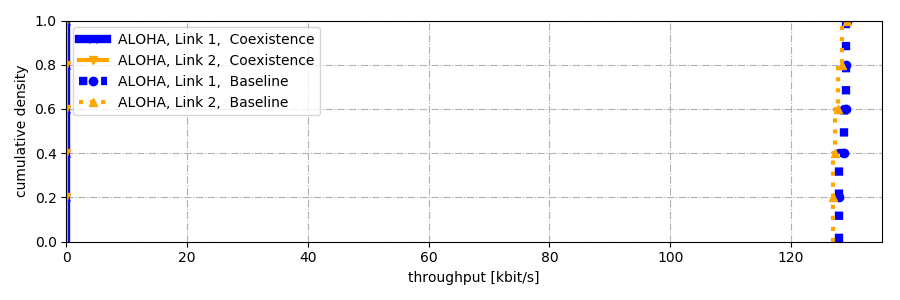
\includegraphics[width=0.9\textwidth]{pictures/results/same_combinations/aloha/throughput_cdf}
	\end{center}
	\caption{Throughput for two links with ALOHA.}
\end{figure}

\begin{figure}[tb]
	\label{fig:results-aloha-dbl-packet-loss}
	\begin{center}
		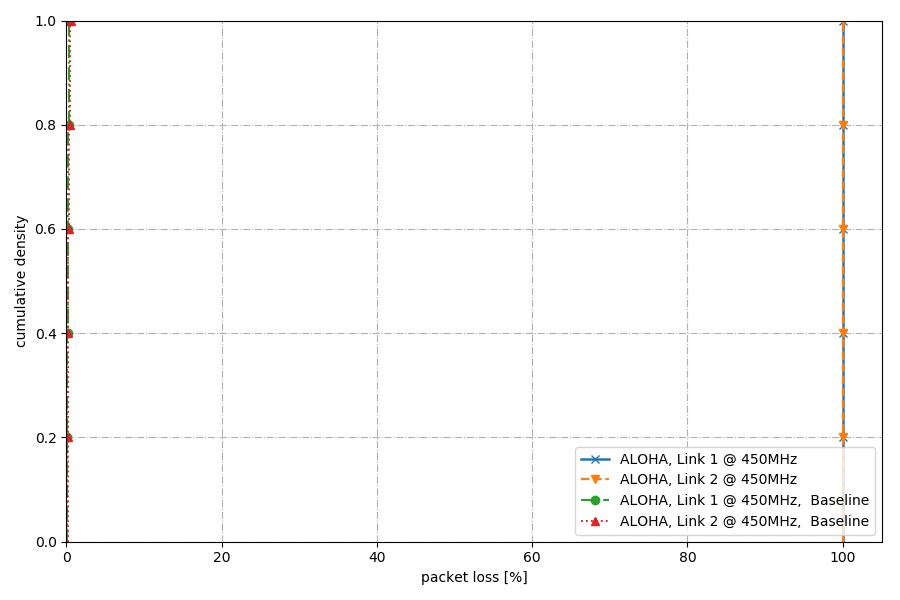
\includegraphics[width=0.9\textwidth]{pictures/results/same_combinations/aloha/packet_loss_cdf}
	\end{center}
	\caption{Packet loss for two links with ALOHA.}
\end{figure}

\begin{figure}[tb]
	\label{fig:results-aloha-dbl-channel-meta}
	\begin{center}
		\subfloat[channel energy CDF]{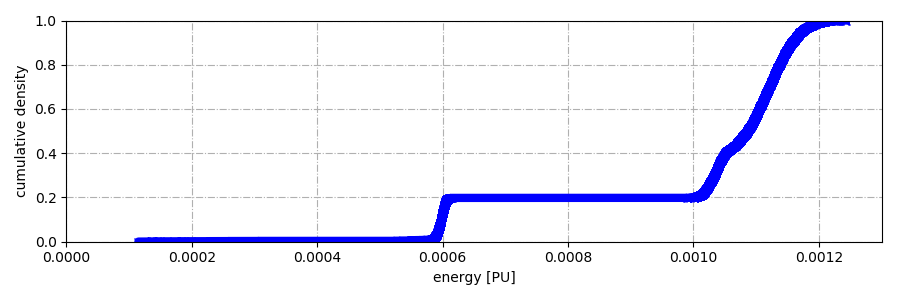
\includegraphics[width=0.9\textwidth]{pictures/results/same_combinations/aloha/smoothed_channel_energy_cdf}\label{fig:results-aloha-dbl-channel-energy-cdf}}
		\\
		\subfloat[channel energy]{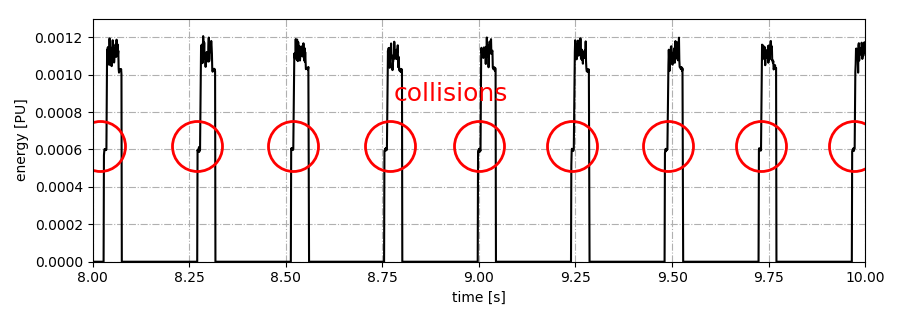
\includegraphics[width=0.9\textwidth]{pictures/results/same_combinations/aloha/smoothed_channel_energy_level_4_line_chart}\label{fig:results-aloha-dbl-channel-energy}}	
	\end{center}
	\caption{Observed channel energy for two links with ALOHA.}
\end{figure}

For two links with saturated ALOHA traffic we expect zero aggregate throughput, since each and every packet collides. Figure \ref{fig:results-aloha-dbl-throughput} confirms this assumption, since both links have zero individual throughput. The corresponding packet loss of 100\% is depicted in Figure \ref{fig:results-aloha-dbl-packet-loss}. A reference value that can be read off Figure \ref{fig:results-aloha-dbl-throughput} is the throughput of a standalone saturated ALOHA link, which is about 130 kbps. This means that the combined throughput of multiple nodes in this channel with the same underlying PHY layer can never exceed 130 kbps and we can assess how well different protocols coexist and how much efficiently they make use of the channel by comparing their aggregated throughput to this value.

Furthermore, a physical view on the channel from the sniffer's perspective is provided in Figure \ref{fig:results-aloha-dbl-channel-meta}\subref{fig:results-aloha-dbl-channel-energy}. Due to the fact that the two transmissions of the senders are not completely overlapping we can see that we do not have a single sender with observed transmission energy level around 0.0011 PU, but instead two transmitters, where the observed energy level of the first transmitter is around 0.0006 PU, which the channel energy CDF in Figure \ref{fig:results-aloha-dbl-channel-meta}\subref{fig:results-aloha-dbl-channel-energy-cdf} confirms. Note that the share of this particular energy (0.0006 PU) in the CDF is so high, because the transmission overlap does not stay constant throughout the whole measurement, but slightly varies with each repetition.

\clearpage

\subsection{CSMA/CA With High Parameter Values}

\begin{figure}[tb]
	\label{fig:results-csma-high-dbl-throughput}
	\begin{center}
		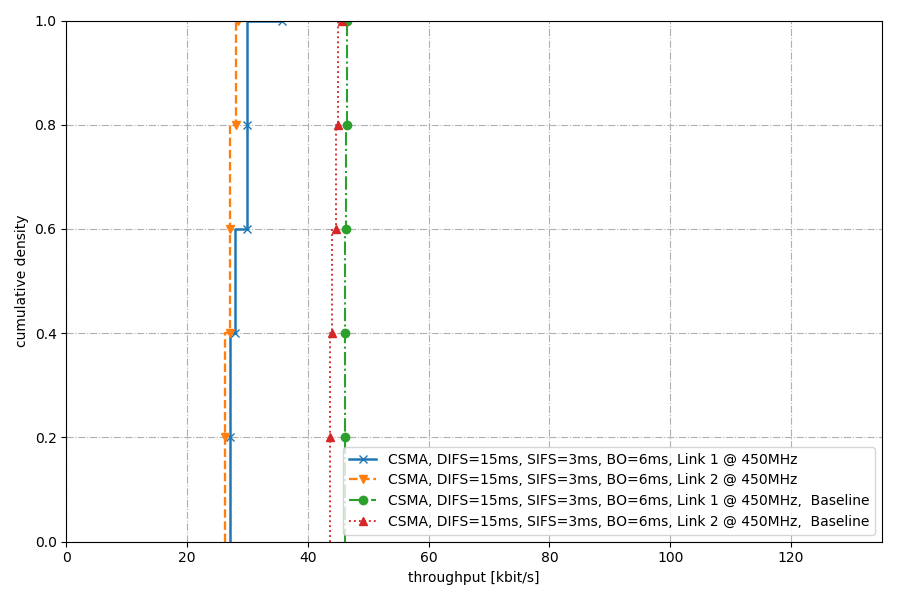
\includegraphics[width=0.9\textwidth]{pictures/results/same_combinations/csma_high_params/throughput_cdf}
	\end{center}
	\caption{Throughput for two links with the high parameter CSMA/CA variant.}
\end{figure}

\begin{figure}[tb]
	\label{fig:results-csma-high-dbl-frame-delay}
	\begin{center}
		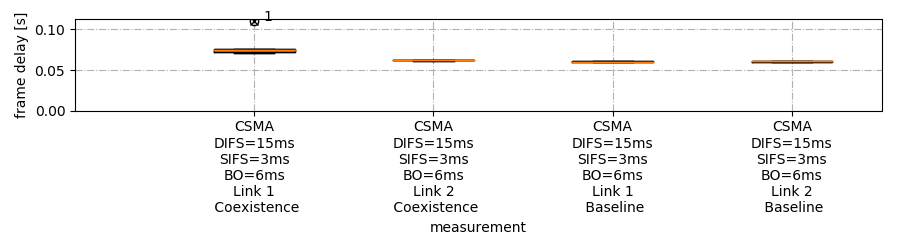
\includegraphics[width=0.9\textwidth]{pictures/results/same_combinations/csma_high_params/frame_delay_boxplot}
	\end{center}
	\caption{Frame delay for two links with the high parameter CSMA/CA variant.}
\end{figure}

\begin{figure}[tb]
	\label{fig:results-csma-high-dbl-backoff}
	\begin{center}
		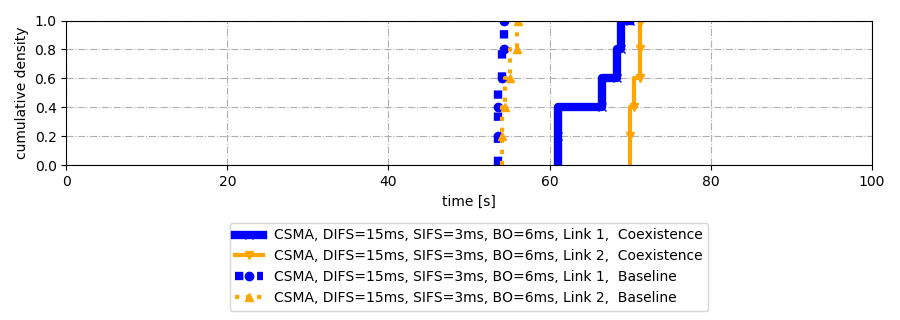
\includegraphics[width=0.9\textwidth]{pictures/results/same_combinations/csma_high_params/backoff_(joint)_sum_cdf}
	\end{center}
	\caption{Backoff for two links with the high parameter CSMA/CA variant.}
\end{figure}

\begin{figure}[tb]
	\label{fig:results-csma-high-dbl-channel-meta}
	\begin{center}
		\subfloat[channel energy CDF]{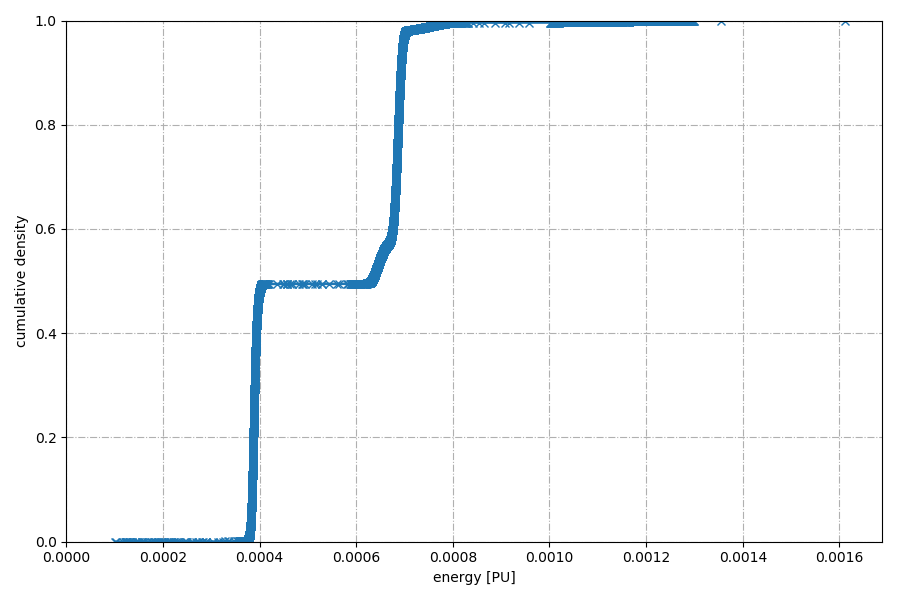
\includegraphics[width=0.9\textwidth]{pictures/results/same_combinations/csma_high_params/smoothed_channel_energy_cdf}\label{fig:results-csma-high-dbl-channel-energy}}
		\\
		\subfloat[channel energy]{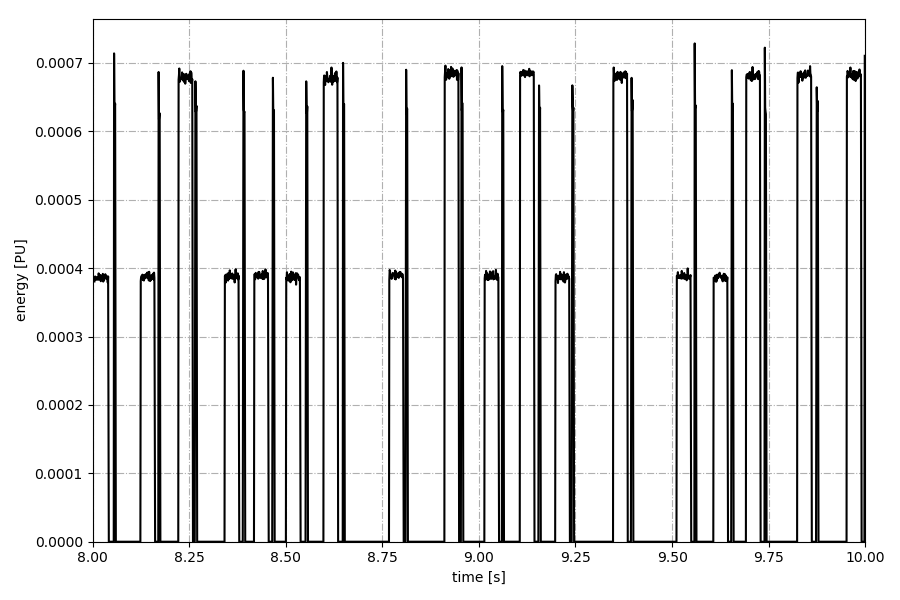
\includegraphics[width=0.9\textwidth]{pictures/results/same_combinations/csma_high_params/smoothed_channel_energy_level_4_line_chart}\label{fig:results-csma-high-dbl-channel-energy-cdf}}
		\\
		\subfloat[logical channel occupation]{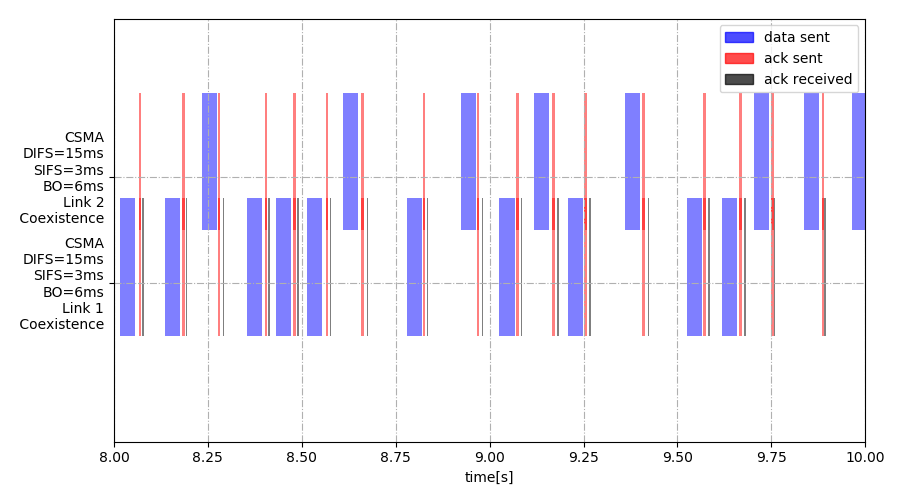
\includegraphics[width=0.9\textwidth]{pictures/results/same_combinations/csma_high_params/zoomed_channel_occupation_gantt_chart}\label{fig:results-csma-high-dbl-channel-occupation}}
	\end{center}
	\caption{Observed channel energy for two links with the high parameter CSMA/CA variant.}
\end{figure}


First of all, with "high parameter values" we mean we chose high values for DIFS, SIFS and backoff slot time (BO), from which we expected that they lead to good coexistence of the two links. In particular, we chose $\text{DIFS}=15 \,\text{ms}$, $\text{SIFS}=3 \,\text{ms}$, $\text{BO}=6 \,\text{ms}$. Figure \ref{fig:results-csma-high-dbl-throughput} shows that the throughput roughly halves (from ) when two links are active at the same time. Figure \ref{fig:results-csma-high-dbl-frame-delay} shows that the frame delay roughly stays the same, where the deviation of the first link comes from packet loss related to hardware problems as described in Section \ref{sec:quality-standards}. Figures \ref{fig:results-csma-high-dbl-channel-meta}\subref{fig:results-csma-low-dbl-channel-energy-cdf}\subref{fig:results-csma-low-dbl-channel-energy} illustrate the same from the sniffer's point of view (POV), as the even throughput among senders is reflected in Figure \subref{fig:results-csma-high-dbl-channel-energy-cdf} with the two observed energy levels of the senders being 0.0004 PU and 0.0007 PU, which is confirmed by Figure \ref{fig:results-csma-high-dbl-channel-energy}. Figure \ref{fig:results-csma-high-dbl-backoff} shows the cumulative backoff times and the logical channel occupation which corresponds to the channel energy plot in Figure \ref{fig:results-csma-high-dbl-channel-meta} \subref{fig:results-csma-high-dbl-channel-energy}. 

\clearpage

\subsection{CSMA/CA With Low Parameter Values}
\label{sec:csma-dbl-low}

\begin{figure}[tb]
	\label{fig:results-csma-low-dbl-throughput}
	\begin{center}
		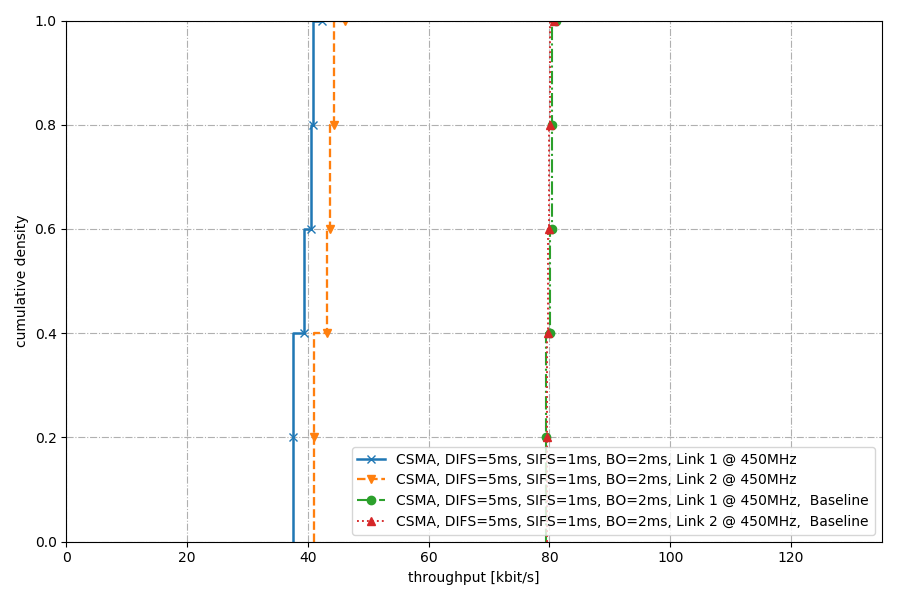
\includegraphics[width=0.9\textwidth]{pictures/results/same_combinations/csma_low_params/throughput_cdf}
	\end{center}
	\caption{Throughput for two links with the low parameter CSMA/CA variant.}
\end{figure}

\begin{figure}[tb]
	\label{fig:results-csma-low-dbl-frame-delay}
	\begin{center}
		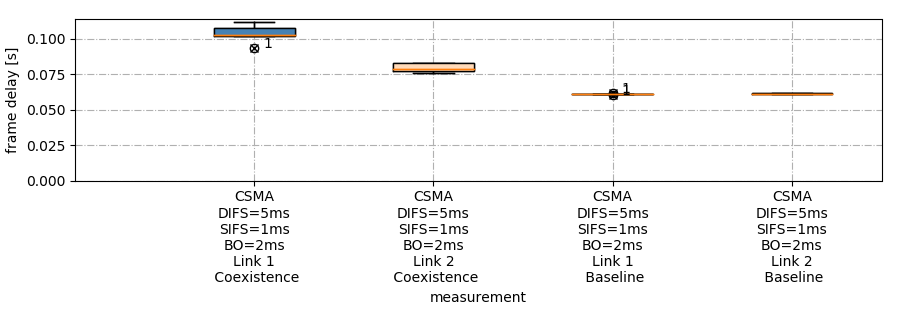
\includegraphics[width=0.9\textwidth]{pictures/results/same_combinations/csma_low_params/frame_delay_boxplot}
	\end{center}
	\caption{Frame delay for two links with the low parameter CSMA/CA variant.}
\end{figure}

\begin{figure}[bt]
	\label{fig:results-csma-low-dbl-backoff}
	\begin{center}
		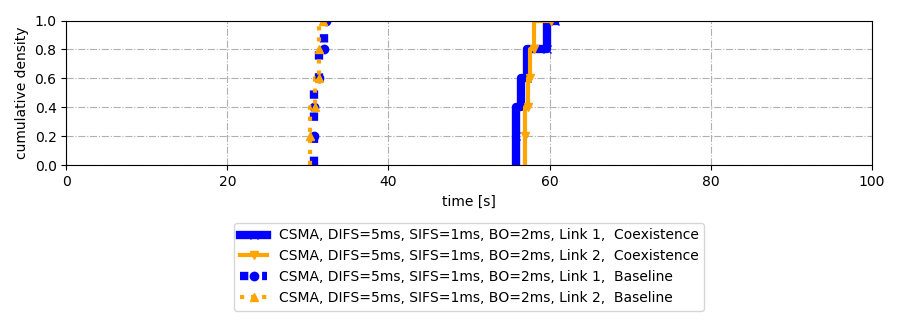
\includegraphics[width=0.9\textwidth]{pictures/results/same_combinations/csma_low_params/backoff_(joint)_sum_cdf}
	\end{center}
	\caption{Backoff times for two links with the low parameter CSMA/CA variant.}
\end{figure}


\begin{figure}[bt]
	\label{fig:results-csma-low-dbl-channel-meta}
	\begin{center}
		\subfloat[channel energy CDF]{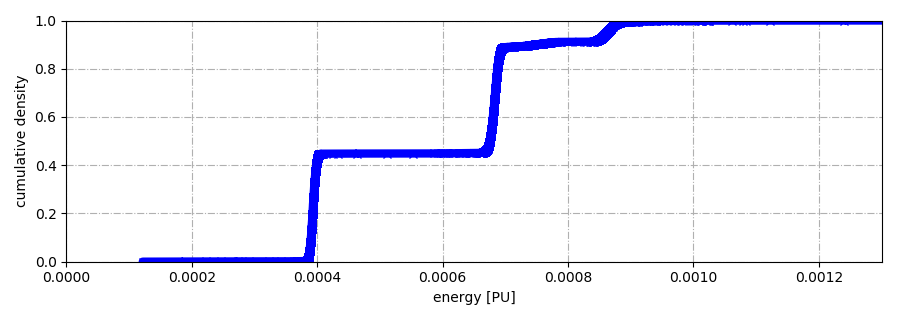
\includegraphics[width=0.9\textwidth]{pictures/results/same_combinations/csma_low_params/smoothed_channel_energy_cdf}\label{fig:results-csma-low-dbl-channel-energy-cdf}}
		\\
		\subfloat[channel energy]{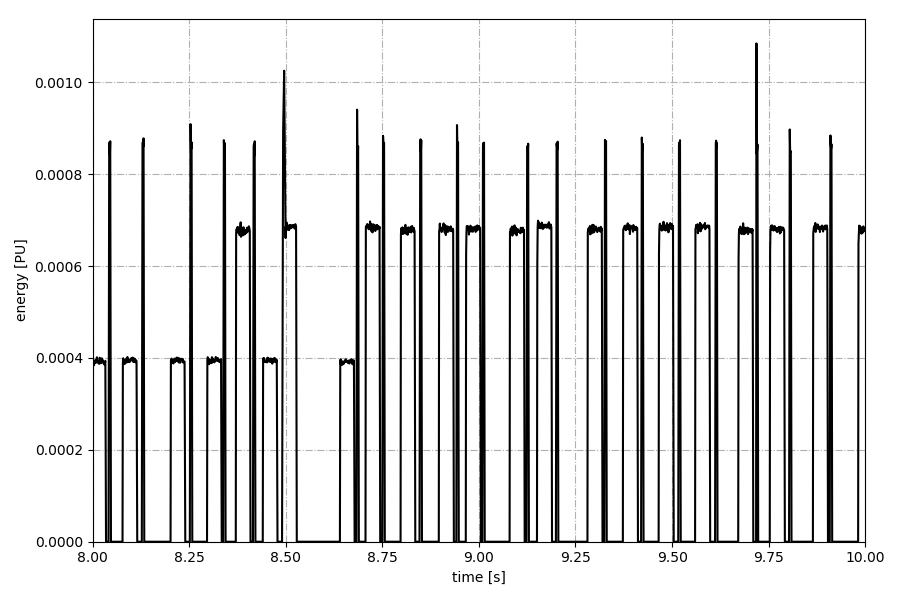
\includegraphics[width=0.9\textwidth]{pictures/results/same_combinations/csma_low_params/smoothed_channel_energy_level_4_line_chart}\label{fig:results-csma-low-dbl-channel-energy}}
		\\
		\subfloat[logical channel occupation]{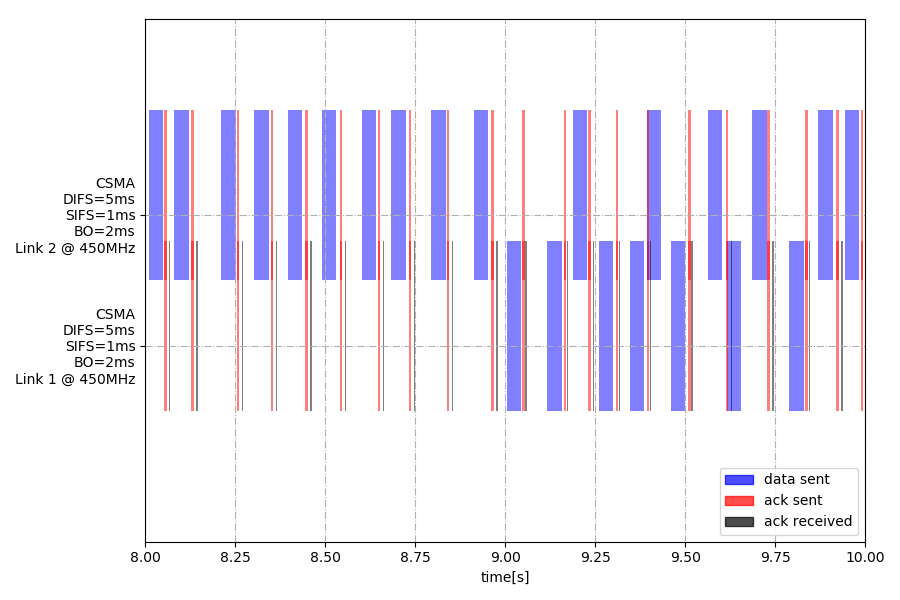
\includegraphics[width=0.9\textwidth]{pictures/results/same_combinations/csma_low_params/zoomed_channel_occupation_gantt_chart}\label{fig:results-csma-low-dbl-channel-occupation}}
	\end{center}
	\caption{Observed channel energy and logical occupation for two links with the low parameter CSMA/CA variant.}
\end{figure}

The next aspect we were interested in is to what extent we can scale down DIFS, SIFS and BO and still retain collision-free transmission. To this end, we reduced the values to $\text{DIFS}=5 \,\text{ms}$, $\text{SIFS}=1 \,\text{ms}$, $\text{BO}=2 \,\text{ms}$\footnote{We chose these values because they are close to the hardware capabilities in terms of time granularity as observed in practice.}. Reducing these values, especially BO increases the throughput, with $CW_\text{min} = 32 \cdot BO$ and uniformly distributed random choice of the backoff slot, we expect a mean delay of $16\cdot BO=32ms$ in the first backoff round, which is rather large compared to DIFS and SIFS.

 Indeed, comparing throughput using the high parameter values (Figure \ref{fig:results-csma-high-dbl-throughput}) with the low parameter values (Figure \ref{fig:results-csma-high-dbl-throughput}) yields a little less than doubled throughput for cutting the backoff. 
 A problem are collisions of ACKs and consecutive data frames of the sender to whom the ACK was not destined caused by the low DIFS in conjunction with hardware delays. Multiple of these collisions occur in the time window depicted in Figure \ref{fig:results-csma-low-dbl-channel-meta}\subref{fig:results-csma-low-dbl-channel-energy}. These collisions lead to the increased frame delays of Figure \ref{fig:results-csma-low-dbl-frame-delay}, where again the additional packet loss of link 1 reflected in the 20ms increased frame delay compared to link 1 is caused by the hardware problems described in Section \ref{sec:quality-standards}.

\clearpage

\subsection{CSMA/CA With Medium Parameter Values}

\begin{figure}[tb]
	\label{fig:results-csma-med-dbl-throughput}
	\begin{center}
		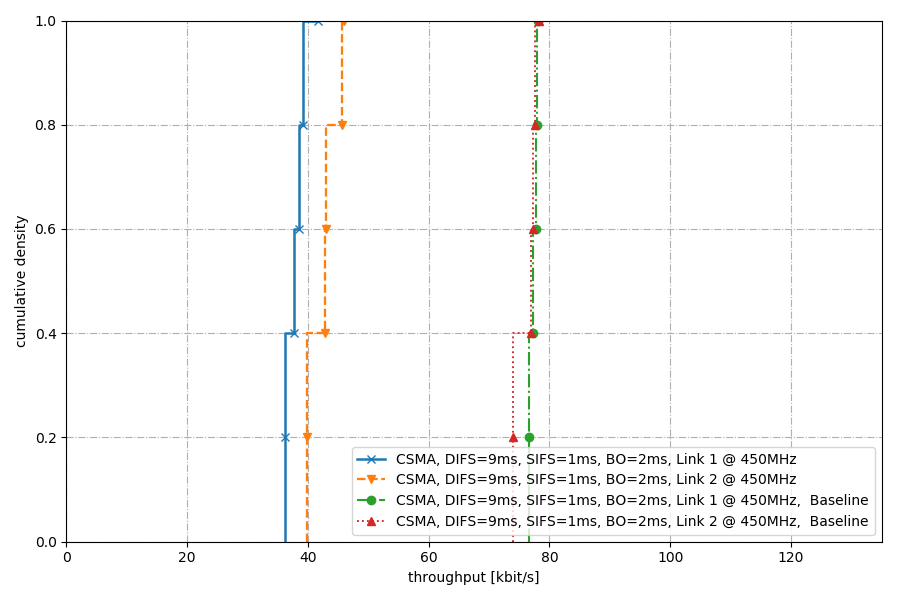
\includegraphics[width=0.9\textwidth]{pictures/results/same_combinations/csma_med_params/throughput_cdf}
	\end{center}
	\caption{Throughput for two links with the medium parameter CSMA/CA variant.}
\end{figure}

\begin{figure}[tb]
	\label{fig:results-csma-med-dbl-frame-delay}
	\begin{center}
		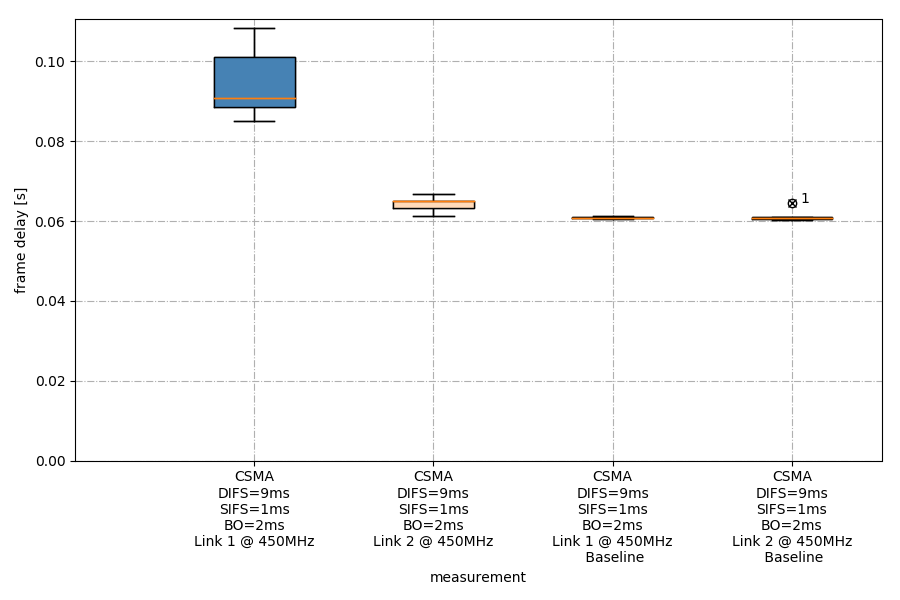
\includegraphics[width=0.9\textwidth]{pictures/results/same_combinations/csma_med_params/frame_delay_boxplot}
	\end{center}
	\caption{Frame delay for two links with the medium parameter CSMA/CA variant.}
\end{figure}

\begin{figure}[tb]
	\label{fig:results-csma-med-dbl-backoff}
	\begin{center}
		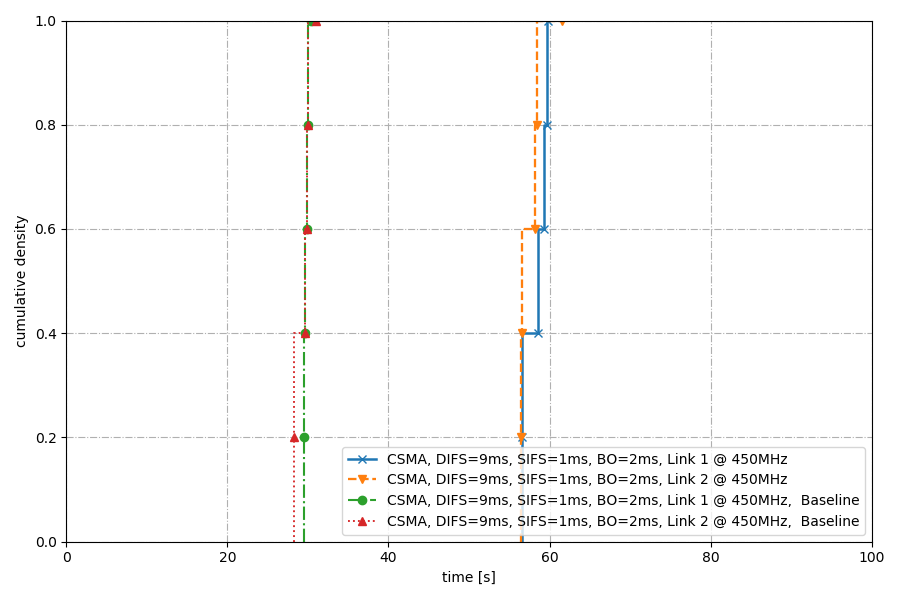
\includegraphics[width=0.9\textwidth]{pictures/results/same_combinations/csma_med_params/backoff_(joint)_sum_cdf}
	\end{center}
	\caption{Backoff times for two links with the medium parameter CSMA/CA variant.}
\end{figure}

\begin{figure}[tb]
	\label{fig:results-csma-med-dbl-channel-meta}
	\begin{center}
		\subfloat[channel energy CDF]{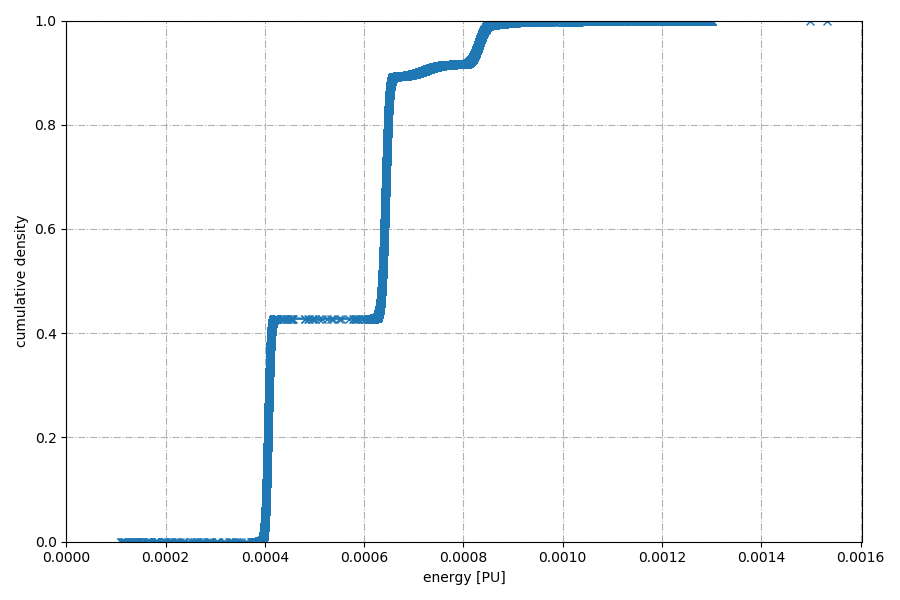
\includegraphics[width=0.9\textwidth]{pictures/results/same_combinations/csma_med_params/smoothed_channel_energy_cdf}}
		\\
		\subfloat[channel energy]{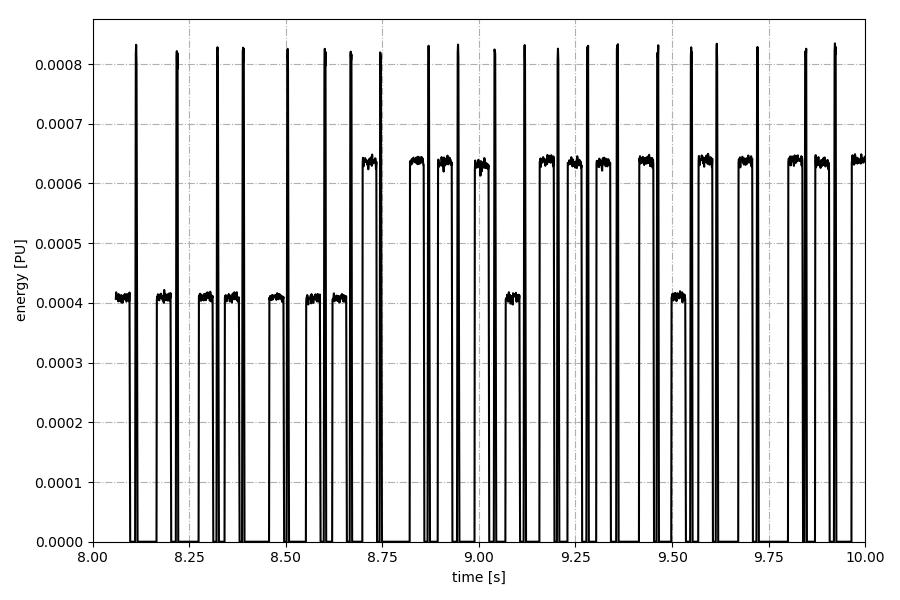
\includegraphics[width=0.9\textwidth]{pictures/results/same_combinations/csma_med_params/smoothed_channel_energy_level_4_line_chart}}
		\\
		\subfloat[logical channel occupation]{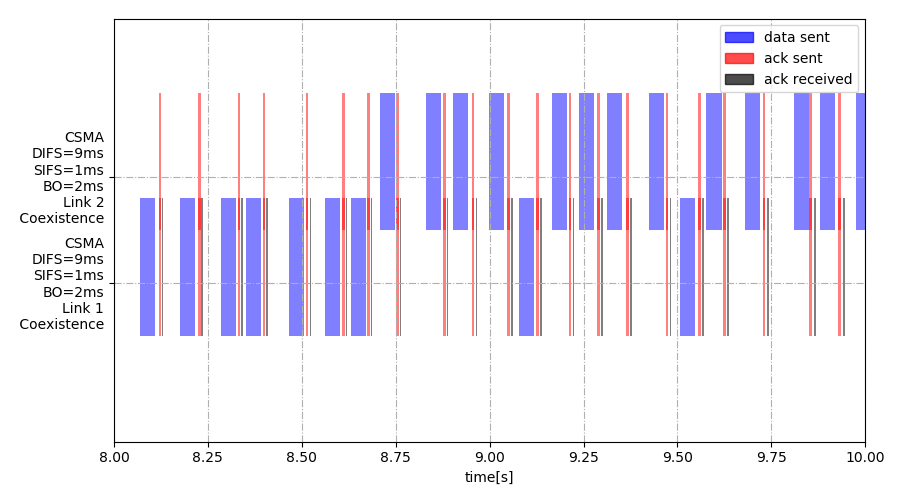
\includegraphics[width=0.9\textwidth]{pictures/results/same_combinations/csma_med_params/zoomed_channel_occupation_gantt_chart}}	
	\end{center}
	\caption{Observed channel energy and logical occupation for two links with the medium parameter CSMA/CA variant.}
\end{figure}

Due to the collisions of ACKs with the data packets of sender 1 as described in Section \ref{sec:csma-dbl-low} we increased DIFS to 9 ms, kept SIFS to 1 ms and BO to 2 ms and indeed, as shown in Figure \ref{fig:results-csma-med-dbl-frame-delay} the frame delay of link 2 is close to the baseline level as result of avoiding collisions. However, since collisions as a result of low DIFS occurred quite infrequently in the last scenario, the metrics (Figures \ref{fig:results-csma-med-dbl-throughput}, \ref{fig:results-csma-med-dbl-backoff}, \ref{fig:results-csma-med-dbl-channel-meta}) roughly stay the same as in the previous scenario (Figures \ref{fig:results-csma-low-dbl-throughput}, \ref{fig:results-csma-low-dbl-backoff}, \ref{fig:results-csma-low-dbl-channel-meta}).

\clearpage

\subsection{1-persistent CSMA}

\begin{figure}[tb]
	\label{fig:results-difs-only-dbl-throughput}
	\begin{center}
		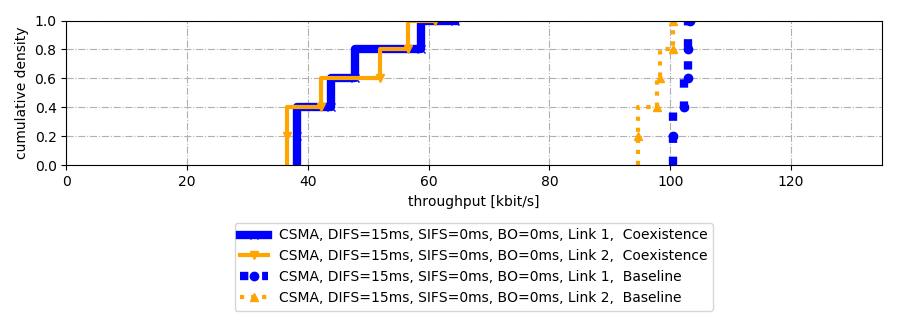
\includegraphics[width=0.9\textwidth]{pictures/results/same_combinations/difs_only/throughput_cdf}
	\end{center}
	\caption{Throughput for two links with 1-persistent CSMA.}
\end{figure}

\begin{figure}[tb]
	\label{fig:results-difs-only-dbl-frame-delay}
	\begin{center}
		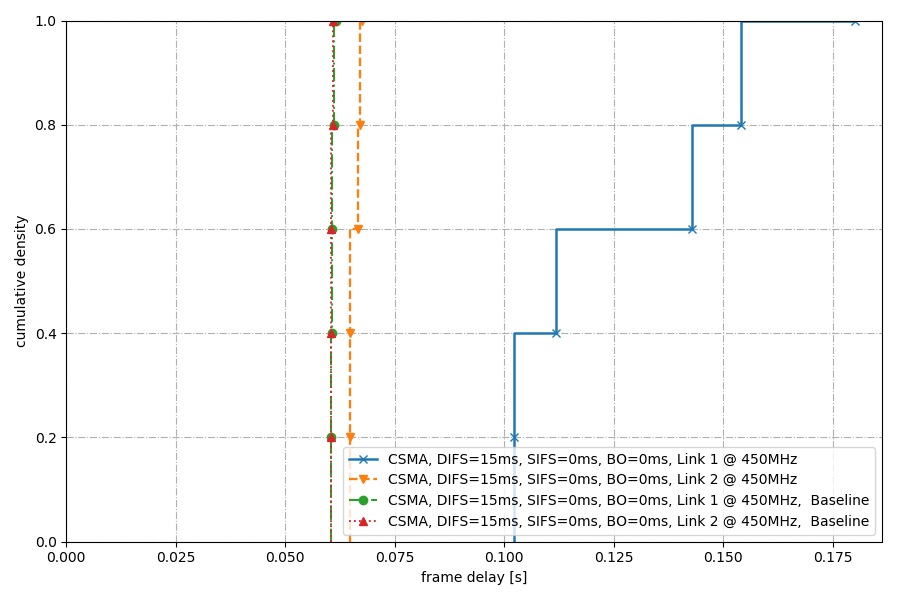
\includegraphics[width=0.9\textwidth]{pictures/results/same_combinations/difs_only/frame_delay_cdf}
	\end{center}
	\caption{Frame delay for two links with 1-persistent CSMA.}
\end{figure}

\begin{figure}[tb]
	\label{fig:results-difs-only-dbl-packet-loss}
	\begin{center}
		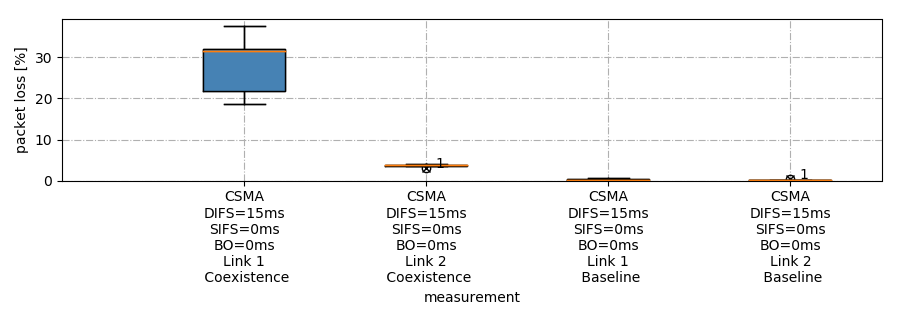
\includegraphics[width=0.9\textwidth]{pictures/results/same_combinations/difs_only/packet_loss_boxplot}
	\end{center}
	\caption{Packet loss for two links with 1-persistent CSMA.}
\end{figure}

\begin{figure}[tb]
	\label{fig:results-difs-only-dbl-channel-meta}
	\begin{center}
		\subfloat[channel energy CDF]{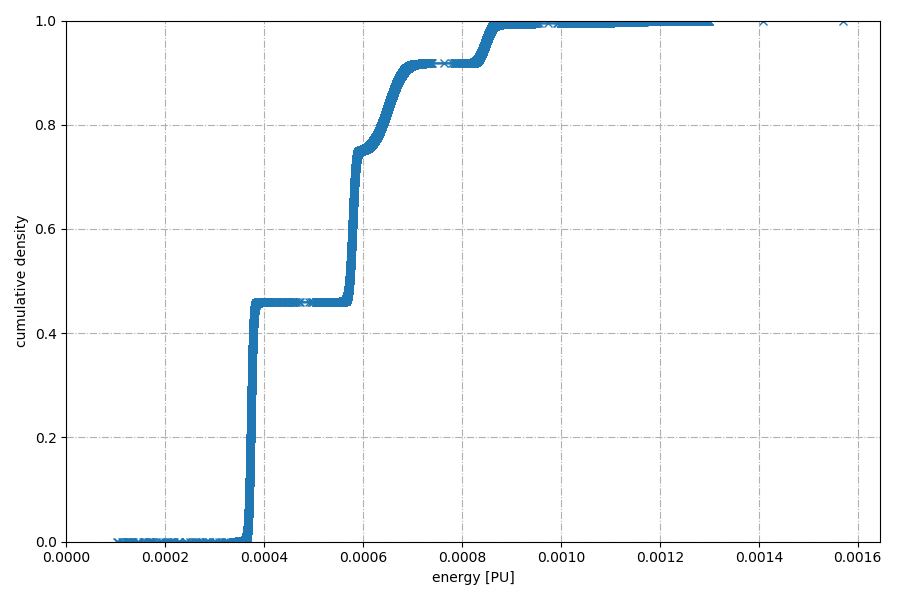
\includegraphics[width=0.9\textwidth]{pictures/results/same_combinations/difs_only/smoothed_channel_energy_cdf}\label{fig:results-difs-only-dbl-channel-energy-cdf}}
		\\
		\subfloat[channel energy]{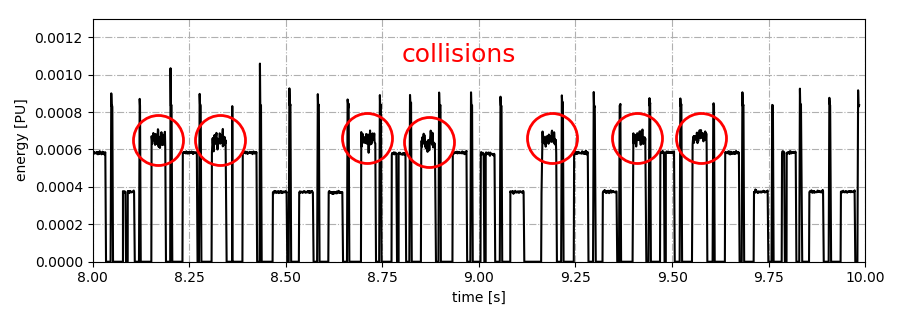
\includegraphics[width=0.9\textwidth]{pictures/results/same_combinations/difs_only/smoothed_channel_energy_level_4_line_chart}\label{fig:results-difs-only-dbl-channel-energy}}
		\\
		\subfloat[logical channel occupation]{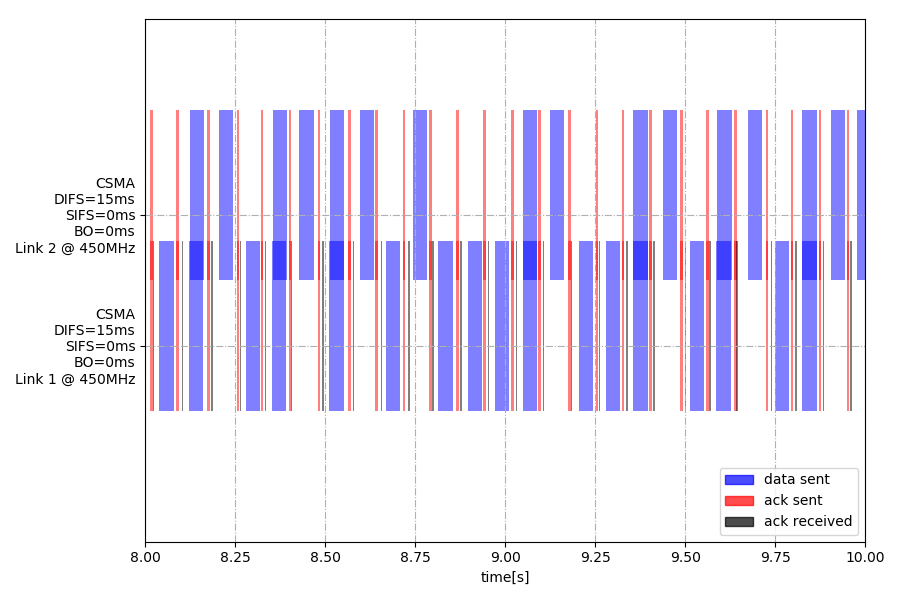
\includegraphics[width=0.9\textwidth]{pictures/results/same_combinations/difs_only/zoomed_channel_occupation_gantt_chart}\label{fig:results-difs-only-dbl-channel-occupation}}
	\end{center}
	\caption{Observed channel energy and logical occupation for two links with 1-persistent CSMA.}
\end{figure}

In the following experiment we examined if a fixed sensing duration of DIFS is enough for harmonious coexistence. As can be seen in Figure \ref{fig:results-difs-only-dbl-channel-meta}\subref{fig:results-difs-only-dbl-channel-occupation} we encounter the problem described in Section \ref{sec:csma-1-persistent}, namely that both\footnote{There are actually three transmitters, since the receiver is transmitting ACKs.} senders try to seize the channel at the same time once a sender finished their transmission. If the time granularity of the system was finer, that is to say its timing accuracy was even higher none of the nodes would start to transmit slightly earlier, leading to even further deteriorated throughput than in Figure \ref{fig:results-difs-only-dbl-throughput}. The higher packet loss (Figure \ref{fig:results-difs-only-dbl-packet-loss}) and thus higher frame delay (Figure \ref{fig:results-difs-only-dbl-frame-delay}) of link 1 compared to link 2  can be elucidated by the fact that the signal-to-interference-plus-noise ratio (SINR) ratio of sender 2 is bigger than the SINR of sender 1\footnote{Also, the SINR of the receiver's ACK signal is higher than all others.} as can be surmised from Figure \ref{fig:results-difs-only-dbl-channel-meta}\subref{fig:results-difs-only-dbl-channel-energy}. The extra bend in the channel energy CDF (Figure \ref{fig:results-difs-only-dbl-channel-meta}\subref{fig:results-difs-only-dbl-channel-energy-cdf}) roughly from 0.0006 to 0.0007 PU is a consequence of the interference which is also very visible in Figure \ref{fig:results-difs-only-dbl-channel-meta}\subref{fig:results-difs-only-dbl-channel-energy}.

\section{Different MAC Protocols For Both Links}
\label{sec:different-protocols}

\subsection{ALOHA and CSMA/CA}
\label{sec:aloha-csma}

\begin{figure}[tb]
	\label{fig:results-aloha-csma-throughput}
	\begin{center}
		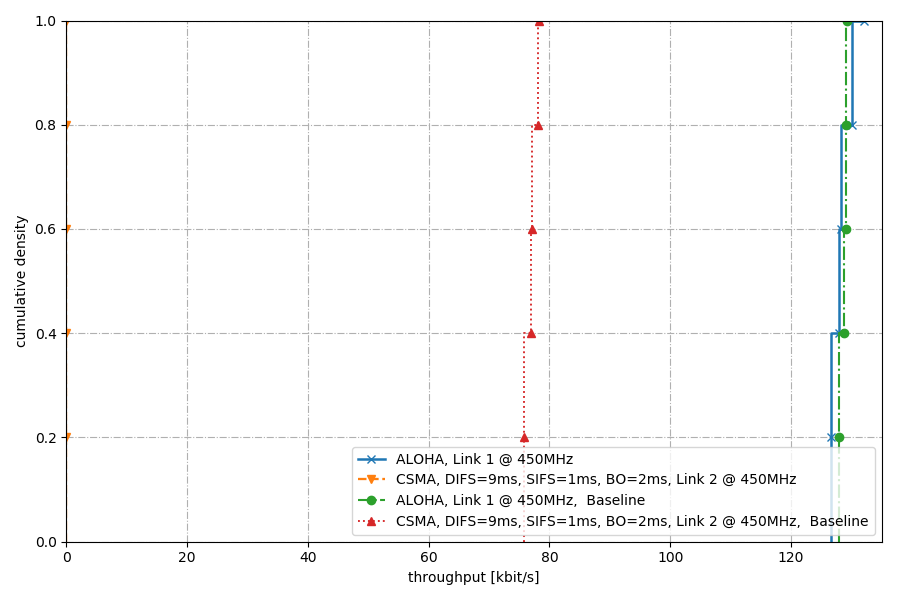
\includegraphics[width=0.9\textwidth]{pictures/results/different_combinations/aloha_csma/throughput_cdf}
	\end{center}
	\caption{Throughput for one link with ALOHA and one link with the medium parameter CSMA/CA variant.}
\end{figure}

\begin{figure}[tb]
	\label{fig:results-aloha-csma-frame-delay}
	\begin{center}
		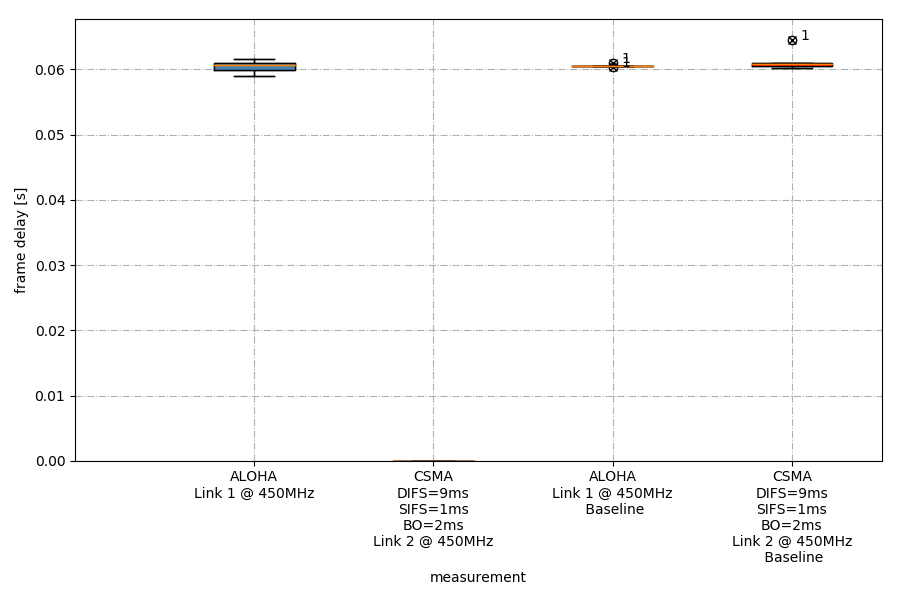
\includegraphics[width=0.9\textwidth]{pictures/results/different_combinations/aloha_csma/frame_delay_boxplot}
	\end{center}
	\caption{Frame delay for one link with ALOHA and one link with the medium parameter CSMA/CA variant.}
\end{figure}

\begin{figure}[tb]
	\label{fig:results-aloha-csma-channel-meta}
	\begin{center}
		\subfloat[channel energy CDF]{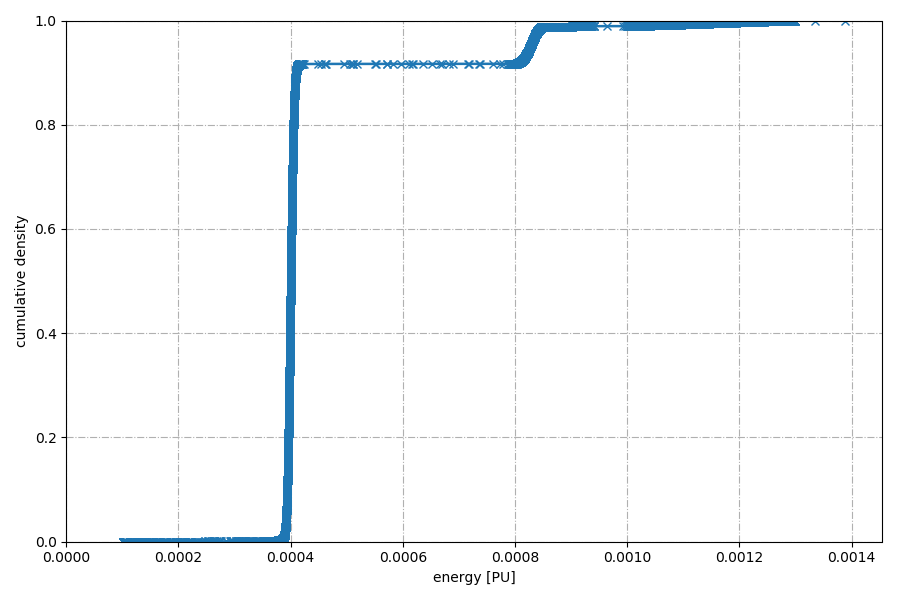
\includegraphics[width=0.9\textwidth]{pictures/results/different_combinations/aloha_csma/smoothed_channel_energy_cdf}\label{fig:results-aloha-csma-channel-energy-cdf}}
		\\
		\subfloat[channel energy]{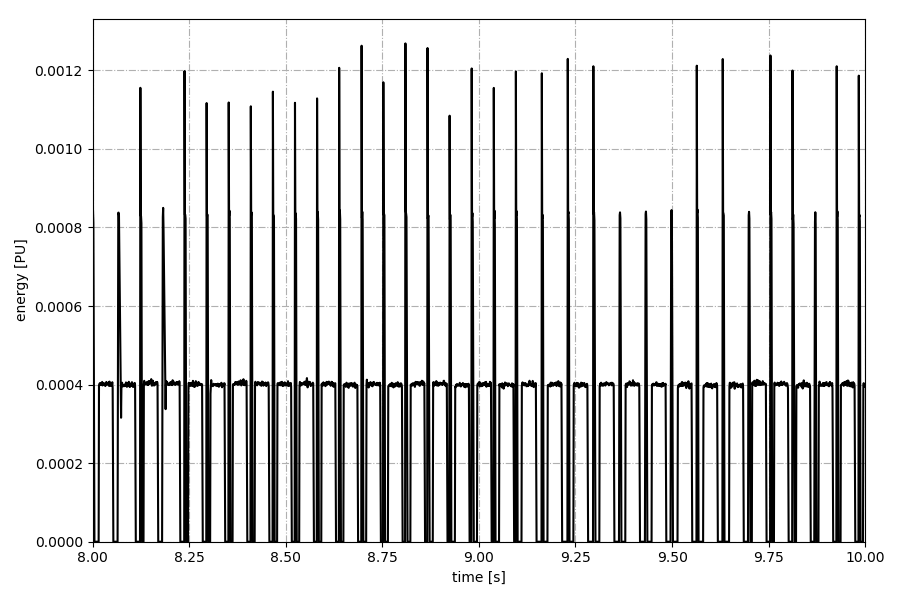
\includegraphics[width=0.9\textwidth]{pictures/results/different_combinations/aloha_csma/smoothed_channel_energy_level_4_line_chart}\label{fig:results-aloha-csma-channel-energy}}
	\end{center}
	\caption{Observed channel energy for one link with ALOHA and one link with the medium parameter CSMA/CA variant.}
\end{figure}

In this experiment we aimed at an experimental confirmation that saturated ALOHA traffic would cause CSMA/CA to stay silent during the whole measurement time. This result is confirmed by Figures \ref{fig:results-aloha-csma-throughput} through \ref{fig:results-aloha-csma-channel-meta}. The throughput and frame delay\footnote{The frame delay is zero, because no frame has ever been sent by the CSMA/CA node.} (Figures \ref{fig:results-aloha-csma-throughput} and \ref{fig:results-aloha-csma-frame-delay}) of CSMA/CA are zero, whereas for saturated ALOHA node throughput and frame delay almost perfectly match the baseline values. The channel energy plots in Figures \ref{fig:results-aloha-csma-channel-meta}\subref{fig:results-aloha-csma-channel-energy} and \ref{fig:results-aloha-csma-channel-meta}\subref{fig:results-aloha-csma-channel-energy-cdf} show that only link 1 and the receiver are transmitting during a time window of 2 s, which also is generally true for the whole measurement duration. 

\clearpage

\subsection{Unsaturated ALOHA and CSMA/CA}
\label{sec:unsat-aloha-csma}

\begin{figure}[tb]
	\label{fig:results-unsat-aloha-csma-throughput}
	\begin{center}
		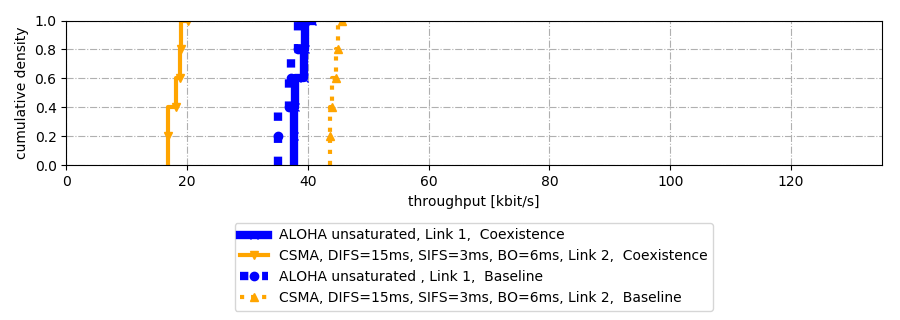
\includegraphics[width=0.9\textwidth]{pictures/results/different_combinations/aloha_unsat_csma/throughput_cdf}
	\end{center}
	\caption{Throughput for one link with unsaturated ALOHA and one link with the high parameter CSMA/CA variant.}
\end{figure}

\begin{figure}[tb]
	\label{fig:results-unsat-aloha-csma-frame-delay}
	\begin{center}
		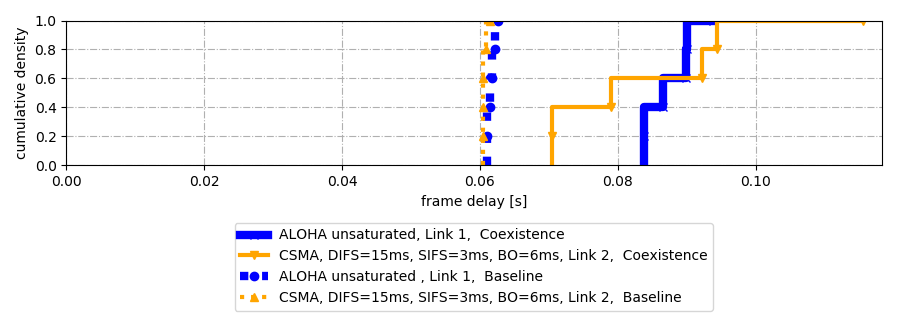
\includegraphics[width=0.9\textwidth]{pictures/results/different_combinations/aloha_unsat_csma/frame_delay_cdf}
	\end{center}
	\caption{Frame delay for one link with unsaturated ALOHA and one link with the high parameter CSMA/CA variant.}
\end{figure}

\begin{figure}[tb]
	\label{fig:results-unsat-aloha-csma-packet-loss}
	\begin{center}
		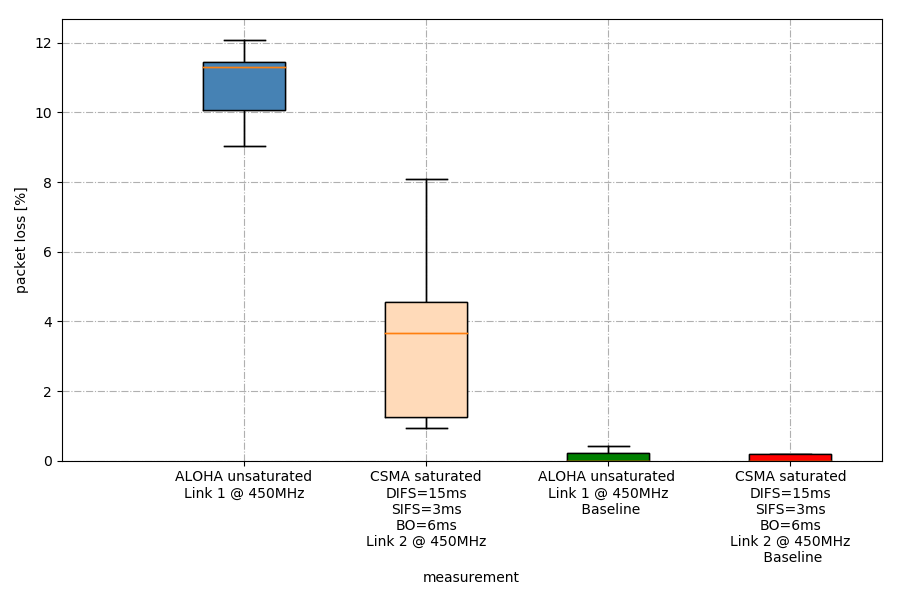
\includegraphics[width=0.9\textwidth]{pictures/results/different_combinations/aloha_unsat_csma/packet_loss_boxplot}	
	\end{center}
	\caption{Packet loss for one link with unsaturated ALOHA and one link with the high parameter CSMA/CA variant.}
\end{figure}

\begin{figure}[tb]
	\label{fig:results-unsat-aloha-csma-channel-meta}
	\begin{center}
		\subfloat[channel energy CDF]{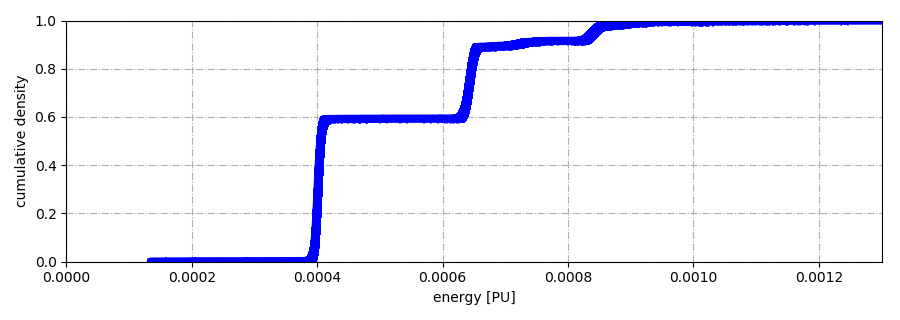
\includegraphics[width=0.9\textwidth]{pictures/results/different_combinations/aloha_unsat_csma/smoothed_channel_energy_cdf}\label{fig:results-unsat-aloha-csma-channel-energy-cdf}}
		\\
		\subfloat[channel energy]{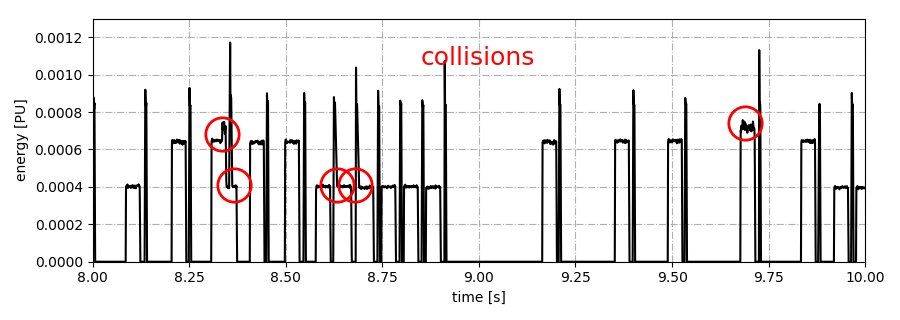
\includegraphics[width=0.9\textwidth]{pictures/results/different_combinations/aloha_unsat_csma/smoothed_channel_energy_level_4_line_chart}\label{fig:results-unsat-aloha-csma-channel-energy}}
		\\
		\subfloat[logical channel occupation]{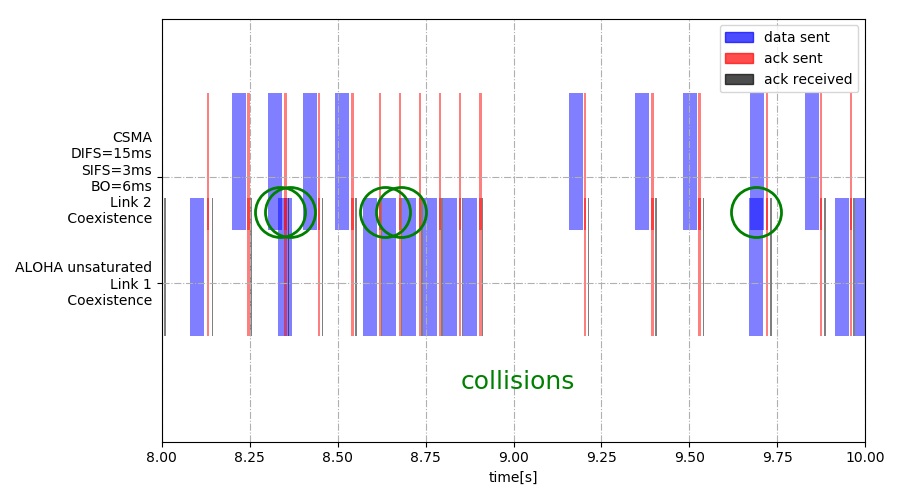
\includegraphics[width=0.9\textwidth]{pictures/results/different_combinations/aloha_unsat_csma/zoomed_channel_occupation_gantt_chart}\label{fig:results-unsat-aloha-csma-channel-occupation}}
	\end{center}
	\caption{Observed channel energy and logical occupation for one link with unsaturated ALOHA and one link with the high parameter CSMA/CA variant.}
\end{figure}

The next experiment investigates whether relatively low load unsaturated\footnote{We still refer to exponentially distributed time between each packet with $\frac{1}{\lambda}=200ms$, which gives us roughly $G_\text{ALOHA,unsat} \approx \frac{38 \text{kbps}}{130 \text{kbps}}\approx 0.3$, where 38 kbps is the baseline throughput of unsaturated ALOHA and 130 kbps the baseline throughput of saturated ALOHA. We can use this approximation, because the offered channel load of ALOHA is independent from other transmitters and saturated ALOHA approximatively consumes the whole channel capacity.} ALOHA can coexist with CSMA/CA. The throughput of the CSMA/CA sender is reduced to $\frac{18}{45}=40\%$ of the baseline value as depicted in Figure \ref{fig:results-unsat-aloha-csma-throughput}, while the ALOHA throughput approximately remains the same.

Only if the CSMA/CA node transmits a frame before the ALOHA node a collision can occur, which happens during seconds 8-10 of the measurement as shown in Figure \ref{fig:results-unsat-aloha-csma-channel-meta}\subref{fig:results-unsat-aloha-csma-channel-occupation} from a logical POV or in Figure \ref{fig:results-unsat-aloha-csma-channel-meta}\subref{fig:results-unsat-aloha-csma-channel-energy} from a physical POV. With that in mind, we can explain why the frame delay of CSMA/CA varies much more than the frame delay of ALOHA (Figure  \ref{fig:results-unsat-aloha-csma-frame-delay}). The number of ALOHA packets generated during data frame transmission time (or any other period of time) is Poisson-distributed and thus the number of collisions, whereas the likelihood of collision from the POV of an ALOHA frame is dependent on the backoff which in our case is uniformly distributed. The same explanation also applies for the differing variances in packet loss as depicted in Figure \ref{fig:results-unsat-aloha-csma-packet-loss}, whereas the differing values are because ALOHA recklessly pushes its packets into channel, while CSMA/CA does not interfere with ALOHA packets when it senses energy in the channel.

\clearpage

\subsection{Two Variants of CSMA/CA}

\begin{figure}[tb]
	\label{fig:results-csma-15-5-throughput}
	\begin{center}
		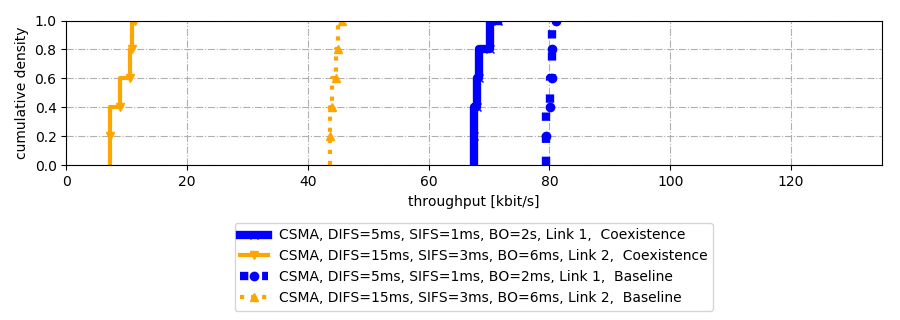
\includegraphics[width=0.9\textwidth]{pictures/results/different_combinations/csma_inhomogeneous/15_5/throughput_cdf}
	\end{center}
	\caption{Throughput for one link with the low parameter CSMA/CA variant and one link with the high parameter CSMA/CA variant.}
\end{figure}

\begin{figure}[tb]
	\label{fig:results-csma-15-5-frame-delay}
	\begin{center}
		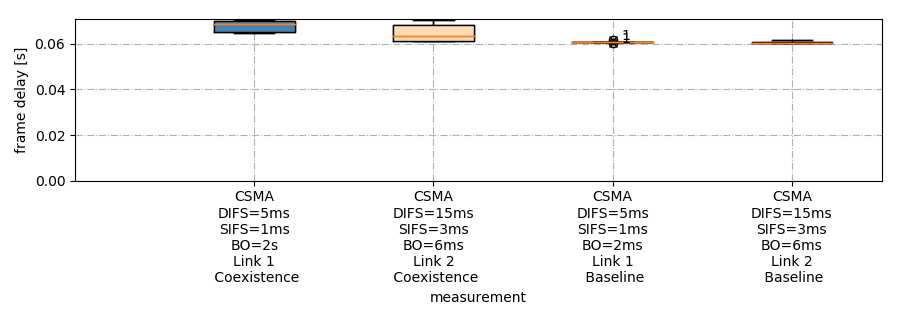
\includegraphics[width=0.9\textwidth]{pictures/results/different_combinations/csma_inhomogeneous/15_5/frame_delay_boxplot}
	\end{center}
	\caption{Frame delay for one link with the low parameter CSMA/CA variant and one link with the high parameter CSMA/CA variant.}
\end{figure}

\begin{figure}[bt]
	\label{fig:results-csma-15-5-packet-loss}
	\begin{center}
		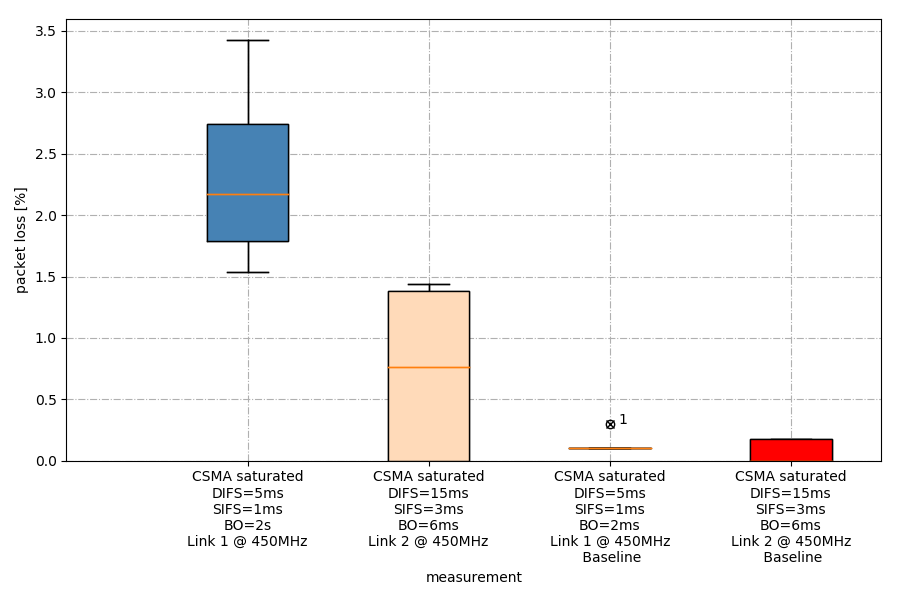
\includegraphics[width=0.9\textwidth]{pictures/results/different_combinations/csma_inhomogeneous/15_5/packet_loss_boxplot}	
	\end{center}
	\caption{Packet loss for one link with the low parameter CSMA/CA variant and one link with the high parameter CSMA/CA variant.}
\end{figure}

\begin{figure}[bt]
	\label{fig:results-csma-15-5-channel-meta}
	\begin{center}
		\subfloat[channel energy CDF]{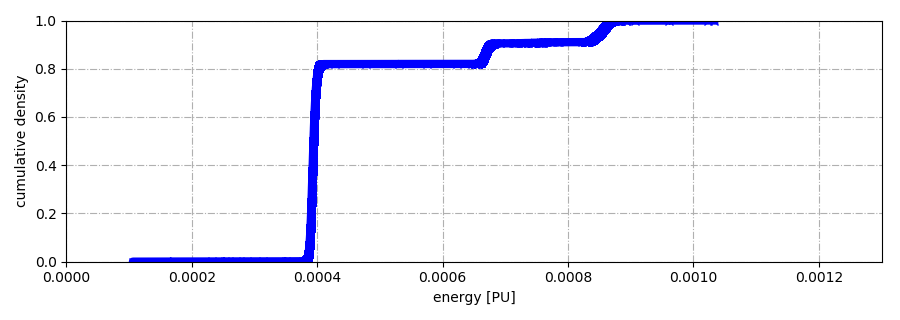
\includegraphics[width=0.9\textwidth]{pictures/results/different_combinations/csma_inhomogeneous/15_5/smoothed_channel_energy_cdf}\label{fig:results-csma-15-5-channel-energy-cdf}}
		\\
		\subfloat[channel energy]{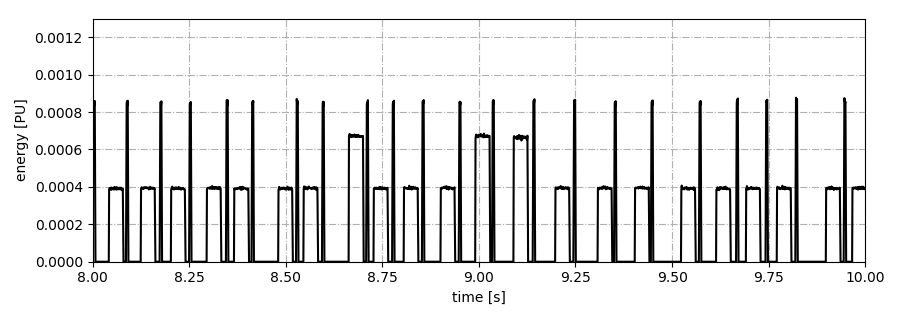
\includegraphics[width=0.9\textwidth]{pictures/results/different_combinations/csma_inhomogeneous/15_5/smoothed_channel_energy_level_4_line_chart}\label{fig:results-csma-15-5-channel-energy}}
		\\
		\subfloat[logical channel occupation]{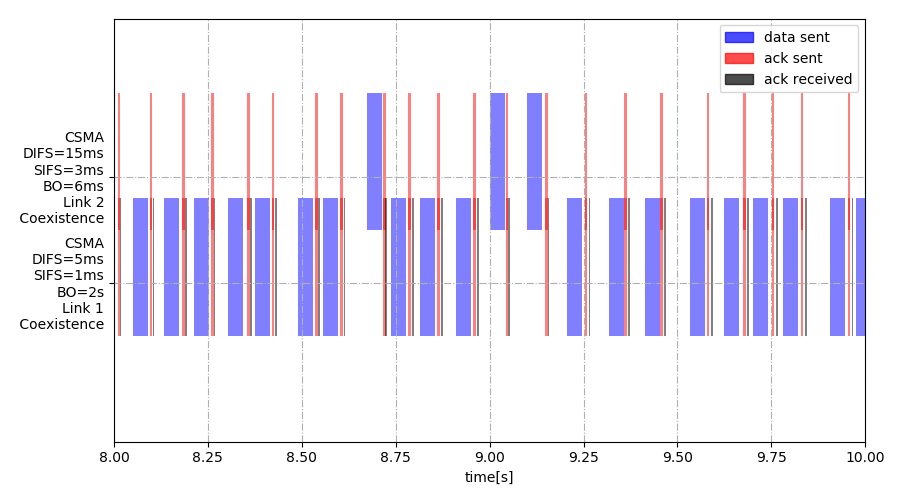
\includegraphics[width=0.9\textwidth]{pictures/results/different_combinations/csma_inhomogeneous/15_5/zoomed_channel_occupation_gantt_chart}\label{fig:results-csma-15-5-channel-occupation}}
	\end{center}
	\caption{Observed channel energy and logical occupation for one link with the low parameter CSMA/CA variant and one link with the high parameter CSMA/CA variant.}
\end{figure}

The goal of our next experiment is to examine how CSMA/CA with different parameter values behave in the same channel. Link 1 uses the low parameter values, whereas link 2 uses the high parameter values. The throughput of link 2 as depicted in Figure \ref{fig:results-csma-15-5-throughput} drops to one seventh of the baseline, whereas it only drops by 20\% for link 1. The reason for this is that with reduced DIFS and BO the chance to grab the channel increases as is shown in Figures \ref{fig:results-csma-15-5-channel-meta}\subref{fig:results-csma-15-5-channel-energy}\subref{fig:results-csma-15-5-channel-energy-cdf}\subref{fig:results-csma-15-5-channel-occupation}. The frame delay increases only marginally as shown in Figure \ref{fig:results-csma-15-5-frame-delay}, which is due to the packet loss depicted in Figure \ref{fig:results-csma-15-5-packet-loss}. The mean packet loss is for link 2 is a little below the expected value of about 1.2\%, whereas for link 1 it is above that value, which is because the SINR of link 2 is higher than for link 1. The expected packet loss comprises of two components. The first component is the baseline packet loss for this measurement, which is around 0.2\%. The second component is the chance that both senders choose the same time to transmit their packet when they sensed the channel idle, which amounts to $ \frac{1}{CW_\text{min}} \cdot \frac{\text{BO}_1}{\text{BO}_2} = \frac{1}{96} \approx 1.0\% $. An idea to reduce the chance of collisions due to this phenomenon is to configure the links to have backoff slot durations that are mutually prime, i.e. have no common divisor, which probably only works if the duration of a backoff slot is big compared to the time granularity of the whole system. 

\clearpage

\subsection{1-persistent CSMA and unsaturated ALOHA}

\begin{figure}[tb]
	\label{fig:results-difs-only-aloha-throughput}
	\begin{center}
		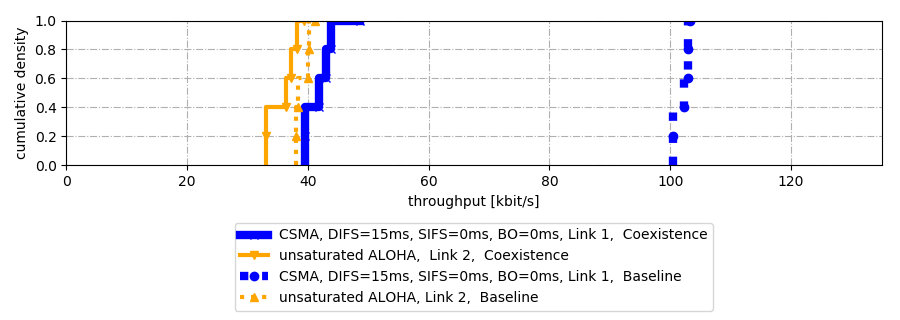
\includegraphics[width=0.9\textwidth]{pictures/results/different_combinations/difs_only_aloha/throughput_cdf}
	\end{center}
	\caption{Throughput for one link with 1-persistent CSMA and one link with unsaturated ALOHA.}
\end{figure}

\begin{figure}[tb]
	\label{fig:results-difs-only-aloha-frame-delay}
	\begin{center}
		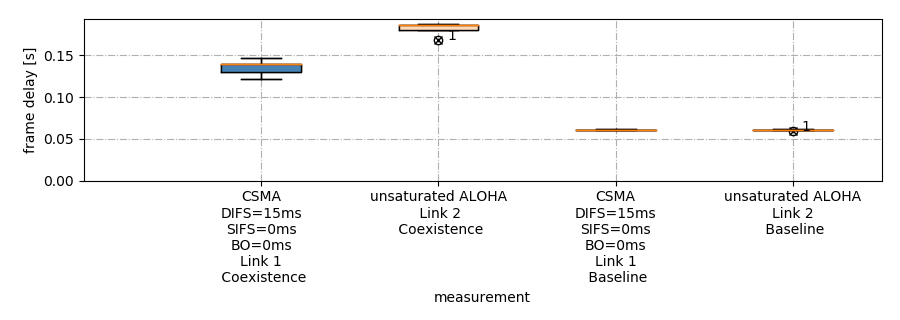
\includegraphics[width=0.9\textwidth]{pictures/results/different_combinations/difs_only_aloha/frame_delay_boxplot}	
	\end{center}
	\caption{Frame delay for one link with 1-persistent CSMA and one link with unsaturated ALOHA.}
\end{figure}

\begin{figure}[bt]
	\label{fig:results-difs-only-aloha-packet-loss}
	\begin{center}
		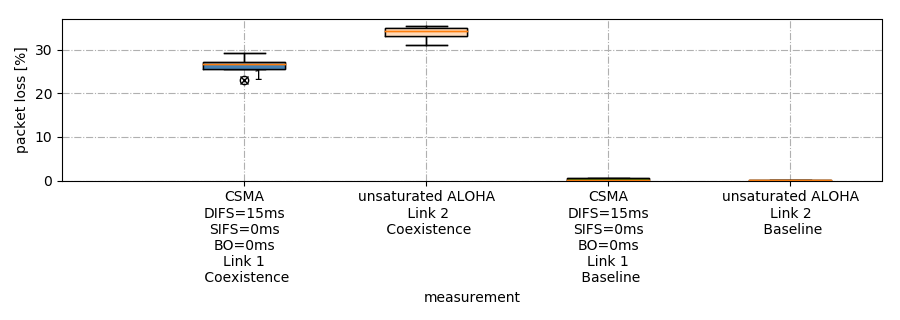
\includegraphics[width=0.9\textwidth]{pictures/results/different_combinations/difs_only_aloha/packet_loss_boxplot}		
	\end{center}
	\caption{Packet loss for one link with 1-persistent CSMA and one link with unsaturated ALOHA.}
\end{figure}

\begin{figure}[bt]
	\label{fig:results-difs-only-aloha-channel-meta}
	\begin{center}
		\subfloat[channel energy CDF]{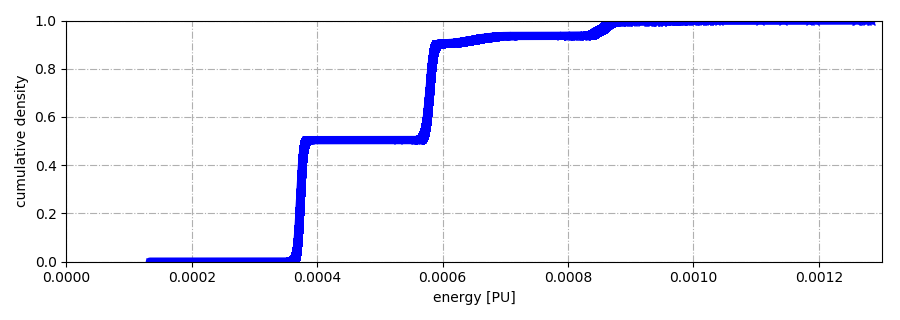
\includegraphics[width=0.9\textwidth]{pictures/results/different_combinations/difs_only_aloha/smoothed_channel_energy_cdf}\label{fig:results-difs-only-aloha-channel-energy-cdf}}
		\\
		\subfloat[channel energy]{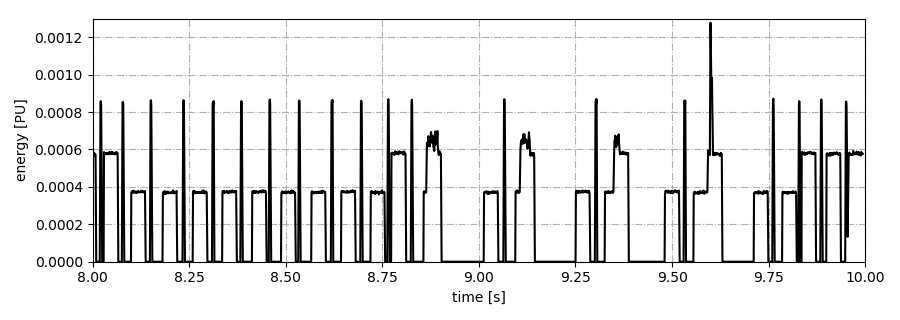
\includegraphics[width=0.9\textwidth]{pictures/results/different_combinations/difs_only_aloha/smoothed_channel_energy_level_4_line_chart}\label{fig:results-difs-only-aloha-channel-energy}}
		\\
		\subfloat[logical channel occupation]{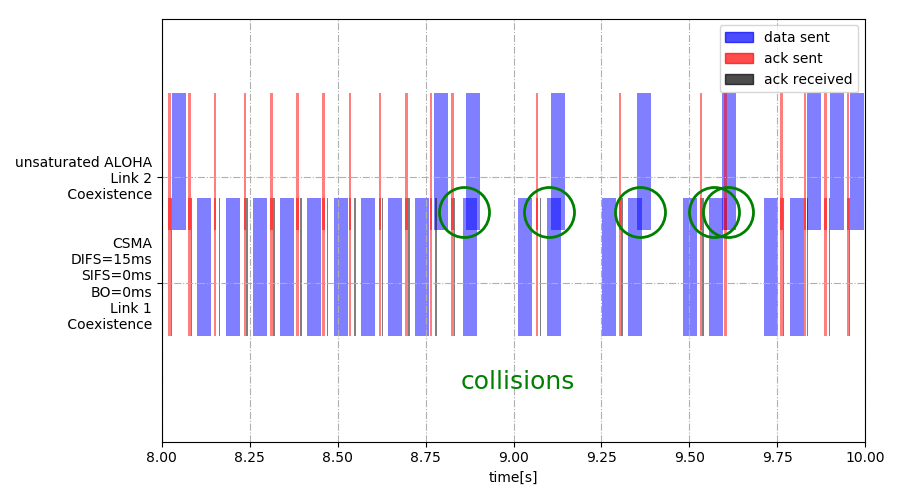
\includegraphics[width=0.9\textwidth]{pictures/results/different_combinations/difs_only_aloha/zoomed_channel_occupation_gantt_chart}\label{fig:results-difs-only-aloha-channel-occupation}}
	\end{center}
	\caption{Observed channel energy and logical occupation for one link with 1-persistent CSMA and one link with unsaturated ALOHA.}
\end{figure}

If there is a link that sends saturated ALOHA traffic through the channel another link will have zero throughput as shown in Sections \ref{sec:dbl-aloha} and \ref{sec:aloha-csma}, which is why we do not consider scenarios with saturated ALOHA traffic anymore. We now discuss a scenario where link 1 uses 1-persistent CSMA and link 2 \emph{unsaturated} ALOHA. In the given scenario it does not make much sense for the CSMA/CA transmitter to back off when the channel is sensed busy either, due to fact that the ALOHA node does not use the LBT mechanism, thus "giving it the chance to transmit" is waste of time as it transmits whenever it wants anyway. Thus, removing the backoff in CSMA/CA promises higher throughput. For this reason we now compare this experiment with the one in Section \ref{sec:unsat-aloha-csma}. The assumption of increased throughput is correct as the comparison between Figures \ref{fig:results-difs-only-aloha-throughput} and \ref{fig:results-aloha-csma-throughput} confirms that removing backoff more than doubles CSMA throughput. It would however, make sense to back off after the reception of an ACK to give the ALOHA node a chance to send a packet. The lack of this backoff explains the increased ALOHA mean packet loss ($\approx 34\%$ total, $\approx 300\%$ increase;  Figure \ref{fig:results-difs-only-aloha-packet-loss}), which is still comparatively low due to the high SINR of the ALOHA node. A representative excerpt of the logical channel occupation is given in Figure \ref{fig:results-difs-only-aloha-channel-meta}\subref{fig:results-difs-only-aloha-channel-occupation}, where only a single ALOHA frame around second 8.8 does not collide with a CSMA packet. The energy plot in Figure  \ref{fig:results-difs-only-aloha-channel-meta}\subref{fig:results-difs-only-aloha-channel-energy} offers a more detailed physical view the channel, where the peak energy level of colliding data packets is not much higher than the energy level of a successful ALOHA transmission. In conjunction with the energy CDF in Figure \ref{fig:results-difs-only-aloha-channel-meta}\subref{fig:results-difs-only-aloha-channel-energy-cdf}, which is taking the whole measurement duration into account and has only a small bend around 0.0006 PU we conclude that if we decrease the TX power of the ALOHA node or use a less robust MCS, such as 64-QAM, ALOHA packet loss would drastically increase. 

\clearpage

\subsection{1-persistent CSMA and CSMA/CA}

\begin{figure}[tb]
	\label{fig:results-difs-only-csma-throughput}
	\begin{center}
		\includegraphics[width=0.9\textwidth]{pictures/results/different_combinations/difs_only_csma/throughput_cdf}
	\end{center}
	\caption{Throughput for one link with 1-persistent CSMA and one link with the high parameter CSMA/CA variant.}
\end{figure}

\begin{figure}[tb]
	\label{fig:results-difs-only-csma-frame-delay}
	\begin{center}
		\includegraphics[width=0.9\textwidth]{pictures/results/different_combinations/difs_only_csma/frame_delay_boxplot}
	\end{center}
	\caption{Frame delay for one link with 1-persistent CSMA and one link with the high parameter CSMA/CA variant.}
\end{figure}

\begin{figure}[tb]
	\label{fig:results-difs-only-csma-channel-meta}
	\begin{center}
		\subfloat[channel energy]{\includegraphics[width=0.9\textwidth]{pictures/results/different_combinations/difs_only_csma/smoothed_channel_energy_level_4_line_chart}\label{fig:results-difs-only-csma-channel-energy}}
		\\
		\subfloat[channel energy CDF]{\includegraphics[width=0.9\textwidth]{pictures/results/different_combinations/difs_only_csma/smoothed_channel_energy_cdf}\label{fig:results-difs-only-csma-channel-energy-cdf}}
	\end{center}
	\caption{Observed channel energy and logical occupation for one link with 1-persistent CSMA and one link with the high parameter CSMA/CA variant.}
\end{figure}

In our last experiment we show that the greedy 1-persistent CSMA approach starves other CSMA/CA links. From the perspective of a CSMA/CA sender it does not matter, whether it shares a channel with a saturated 1-persistent CSMA sender or saturated ALOHA sender (Section \ref{sec:aloha-csma}). We can virtually identify no difference in the metrics (Figures \ref{fig:results-difs-only-csma-frame-delay} and \ref{fig:results-difs-only-aloha-channel-meta}\subref{fig:results-difs-only-csma-channel-energy}\subref{fig:results-difs-only-csma-channel-energy-cdf} compared to the corresponding Figures in Section \ref{sec:aloha-csma}) between those combinations except for the reduced throughput \ref{fig:results-difs-only-csma-channel-meta}\subref{fig:results-difs-only-csma-channel-energy-cdf} due to the addition of channel sensing with the duration of DIFS compared to ALOHA. Only if we decreased the offered load of 1-persistent CSMA we could see any and better coexistence\footnote{compared to ALOHA due to the LBT mechanism that stops the 1-persistent CSMA sender from interfering with ongoing transmissions} with CSMA/CA at all.

